% Chapter 2

\chapter{Methodology and approach} % Write in your own chapter title
\label{Chapter2}

\section{Image analysis tools}
\indent Matlab and OpenCV~\cite{34} are two highly used image processing
tools.  Matlab comes with rich image processing and analysis libraries.
It supports most of the work discussed in chapter ~\ref{Chapter1}.
Matlab also provides interface to convert the code into a C code.
However, generated C code is normally very bulky and takes higher
execution time. OpenCV is an open source computer vision library
initiated by Intel. It is available at
http://SourceForge.net/projects/opencvlibrary. It can be used for
research or even commercial purposes. Unlike GNU Public License (GPL),
its licensing does not force that modifications to the library be made
public. \\
\indent OpenCV has been mainly developed in C and C++ on Linux platform.
However, interfaces for other scripting / programming languages such as
Python, Ruby, Java etc have also been developed. Libraries are also
available for windows, Android and Mac OS platform. OpenCV libraries
have been used in many applications since its first release in 1999.
Range of applications varies from stitching street view images together,
detecting intrusions in surveillance video, monitoring mine equipment,
helping robots navigate and pick up objects, detection of swimming pool
drowning accidents, running interactive art, checking runways for
debris, inspecting labels on products in factories, to rapid face
detection.\\
\indent OpenCV design goal is to build computer vision library with
computational efficiency which can work with real time applications. It
contains functions in almost all the area of image processing  and
computer vision like, histogram processing, morphological processing,
segmentation, detection tracking, camera calibration etc. Therefore,
selection of OpenCV libraries allows faster evaluation and development
of real embedded application.\\
\indent OpenCV libraries are also available for embedded architecture
CPUs like ARM. This allows easy porting of applications developed on x86
platform to ARM or other embedded platforms.\\
\indent Therefore, we decided to implement our image processing
algorithms in C and on Linux platform, so that it can easily be ported
from a PC to embedded environment. Wherever possible, we have used
OpenCV library.
\section{Surveillance image processing flow}
\begin{figure}[!b]
\centering
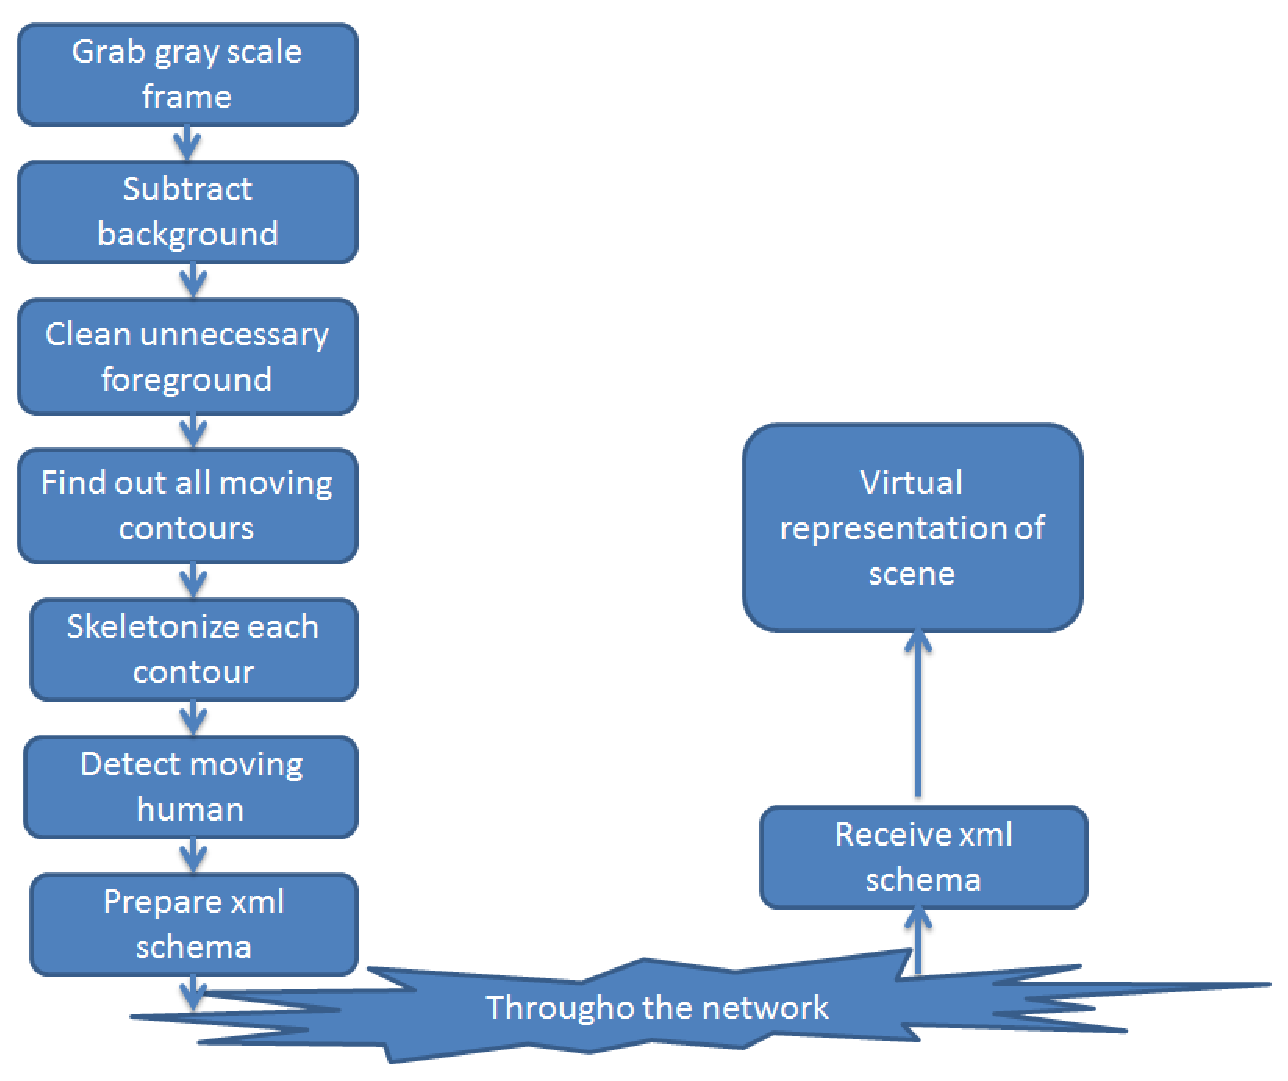
\includegraphics[height=120pt]{Figures/image_pipeline}
\caption{Low BW surveillance image application flow}
\label{image_pipeline}
\end{figure}
\indent Top level surveillance image processing flow for a low bandwidth
network is as shown in Fig.~\ref{image_pipeline}. End goal of low
bandwidth implementation would be to generate information such as human
detected, their position and the time of detection. Therefore, for above
implementation we have to decide on following items, keeping
computational efficiency and true detection for considered object as
primary objective while making any decision.\\
\begin{itemize}
\item \textbf{Background Subtraction:} Methods based on LBP by Yao et
	al.~\cite{11} have striking nice result. It works superbly with
	varied background situation like wavering tree, moving escalator
	etc. Barnich et al.~\cite{9} claim that Vibe which uses random
	sample selection also performs well in all situation and have
	extremely low computational cost. Yao et al. have provided their
	C code, however Barnich et al. have only provided an object
	library for x86 platform. Therefore we need to first code vibe
	in C and then to compare above two algorithms. We did not
	compare other algorithms like GMM, median filter etc with Vibe,
	as authors of Vibe have already done it and concluded that Vibe
	outperforms them.
\item \textbf{Detection and Tracking:} Methods based on skeleton motion
	features~\cite{32, 22, 31} seem to be computationally
	efficient. So we need to evaluate different method of
	skeletonization, suitable for motion calculation. Performance of
	detector based on such method need to be compared with other
	methods based on covariance feature with cascade of logitboost
	classifier~\cite{19}  and Haar-like features~\cite{17} for
	which C code are already available in public domain.
\item \textbf{Embedded implementation:} It is very important to see
	performance of surveillance application based on different
	algorithm on real embedded platform. ARM controller is used in
	most of the embedded multimedia applications. Therefore, it will be
	good to observe their performance with ARM controller.
\end{itemize}
\section {Evaluation of surveillance application techniques}
\subsection{Frame acquisition}
\indent OpenCV provides a way to grab frames either from a camera or
from a file. cvCaptureFromFile or cvCaptureFromCAM returns CvCapture *
struct which can further be used to query frame from either a test video
file or from camera respectively. cvQueryFrame function reads one frame
and returns its pointer. If camera's output or test video is in RGB mode
then, it need to be converted into gray scale image for further
processing. cvCvtColor function has been used to convert image from RGB
to gray scale.
\subsection{Background removal}
\indent Since background subtraction has key role in accomplishing
intended job, therefore we have compared two recently developed~\cite{3,
5} efficient background subtraction algorithm and then selected one of
them~\cite{5} in our final work.  The method described by Yao and
Odobez~\cite{3} is based on use of texture features present in Local
Binary Pattern (LBP).  LBP works well with local illumination changes,
however there can be issues in case of global illumination change. They
have carried out several improvements by using photometric invariant
color measurement and flexible weight updating for background
modes. However, our experiments says that, computationally it is very
less efficient compared to method proposed by Barnich et al.~\cite{9},
which is based on unique way of replacing background pixel value over
the time. It replaces background values for last N frames randomly.
Furthermore, it diffuses updated values to neighbouring pixels, and
again that too on random basis. We have selected method by Barnich et
al.~\cite{9} in our final application, because of its computational
efficiency while maintaining quality.  Fig.~\ref{bg_compare} shows the
comparison of execution time of these two algorithm.

\begin{figure}[!t]
\centering
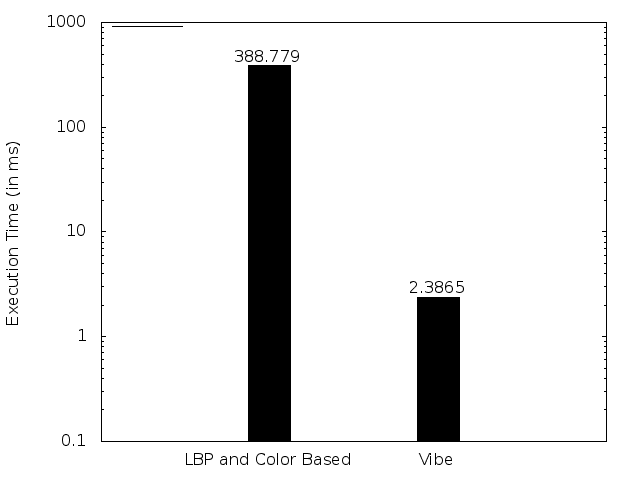
\includegraphics[height=300pt]{Figures/bg_compare}
\caption{Background subtraction average execution time of~\cite{11}
and~\cite{9}. This timing was observed with a x86 system having DMIPS =
800.}
\label{bg_compare}
\end{figure}
\subsection{Noise removal}
\indent None of the background subtraction algorithm allows pure
foreground extraction. There would always be several noise objects in the
extracted image. These are cleaned by morphological erosion operation
(cvErode) followed by dilation (cvDilate) operation. Further all moving
contours are separated out by using OpenCV library function
cvFindContours. This function provides us boundary point of individual
moving object.
\subsection{Skeletonization techniques}
\indent Image skeletons are points on the image, which are equidistant
to their boundaries.  Skeleton is a very effective way to represent
shape of an object.  Shape analysis of an object further leads to
identification of object.  Skeletonization is a process of thinning
object image by maintaining its topology. There are several mathematical
definitions to do this job. We have evaluated different skeletonization
techniques, with their merits and demerits for the suitability to our
requirement.
\begin{itemize}
\item \textbf{Contour skeleton:} When image of an object is represented by
	a single color say black, it is called silhouette. Outer boundary
	points of silhouette connected together is called contour of
	that object. Contour gives idea about global shape of an object.
	cvFindContours gives us all boundary points of a silhouette.
	However, we can analyze the shape even with lower number of
	points. cvApproxPoly can further be used to approximate it into
	polygon. Vertices of this polygon connected together gives an
	idea about outer shape of the object. An example of such
	skeleton has been shown in Fig.~\ref{skeletons}.A.

\begin{figure}[!t]
\centering
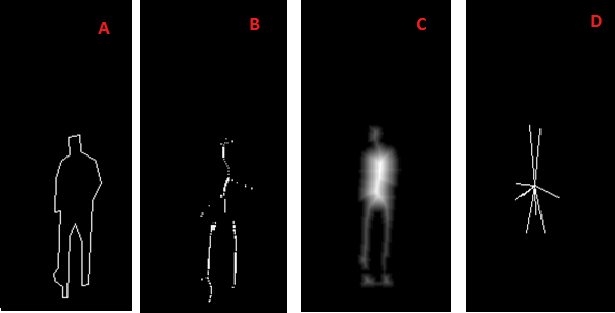
\includegraphics[height=220pt]{Figures/skeletons}
\caption{Skeleton obtained by different methods.\\
	\textbf{A.} Contour skeleton\\
	\textbf{B.} Morphological skeleton\\
	\textbf{C.} Distance transform skeleton\\
	\textbf{D.} Star skeleton}
\label{skeletons}
\end{figure}
\item \textbf{Morphological skeleton:} Morphology is a mathematical
	technique for analysis of structure of any geometry. It was
	mainly defined for the analysis of binary images. Basically, an
	image is probed with a pre-defined shape which is called
	structuring element. Gonzalez and Woods have provided
	a set of morphological operations in their book Digital image
	processing~\cite{35}, where they have defined morphological
	skeletonization as follows:
	\begin{equation}
	\begin{aligned}
		S(A) &= \Sigma ^K _{k = 0} S_k(A) \label{morph_skel}\\
	\mathrm{where} \hspace{5 mm} S_k(A) &= (A \ominus kB) - (A \ominus kB) \circ B \\
			  k &= max \{ K | (A \ominus kB) \neq \phi\}
	\end{aligned}
	\end{equation}
Translating Eqn~\ref{morph_skel} into C code: \par
\fbox{\parbox{\textwidth}{%
	do \\
	\{\\
	\hspace*{1 in}cvErode(img, eroded, element, 1);\\
	\hspace*{1 in}cvDilate(eroded, temp, element, 1);\\
	\hspace*{1 in}cvSub(img, temp, temp, NULL);\\
	\hspace*{1 in}cvOr(skel, temp, skel, NULL);\\
	\hspace*{1 in}cvCopy(eroded, img);\\
	\hspace*{1 in}done = (cvCountNonZero(img) == 0);\\
	\} while (!done);
}} \par
\indent An example of skeleton obtained by morphological method has been
shown in Fig.~\ref{skeletons}.B.
\item \textbf{Skeleton by distance transform:} Distance transform of an
	input image is obtained by creating a new image where pixels are
	set to a value equal to the distance to the nearest zero value
	pixel in input image. We have seen that the contour skeleton
	provided outer shape of the object, where as distance transform
	method provides internal orientation of object. OpenCV provides
	a function cvDistTransform, which can be used to build a
	distance transformed image. An example of skeleton obtained by
	distance transform method has been shown in
	Fig.~\ref{skeletons}.C.
\item \textbf{Star Skeleton:} In this method we plot distance of each
	boundary point from the centroid and then use peaks of the curve
	as skeleton point.
\begin{itemize}
\item Centroid of each object is found out using following
	Eqn~\ref{centroid_calc}.
	\begin{eqnarray}
	C_x = {1 \over N} \Sigma ^N _{i = 1} X_i \label{centroid_calc}
\nonumber \\
	C_y = {1 \over N} \Sigma ^N _{i = 1} Y_i 
	\end{eqnarray}
Here X$_i$ and Y$_i$ are (X,Y) co-ordinates of i$_{th}$ point on the contour
boundary.
\item Distance d$_i$ is calculated between centroid and each boundary
	point as follows. This calculated distance vector are stored in a
	CvMat array.
	\begin{equation}
	d_i = \sqrt{(C_x - X_i)^2 + (C_y - Y_i)^2} \label{dist_calc}
	\end{equation}

\begin{figure}[!t]
\centering
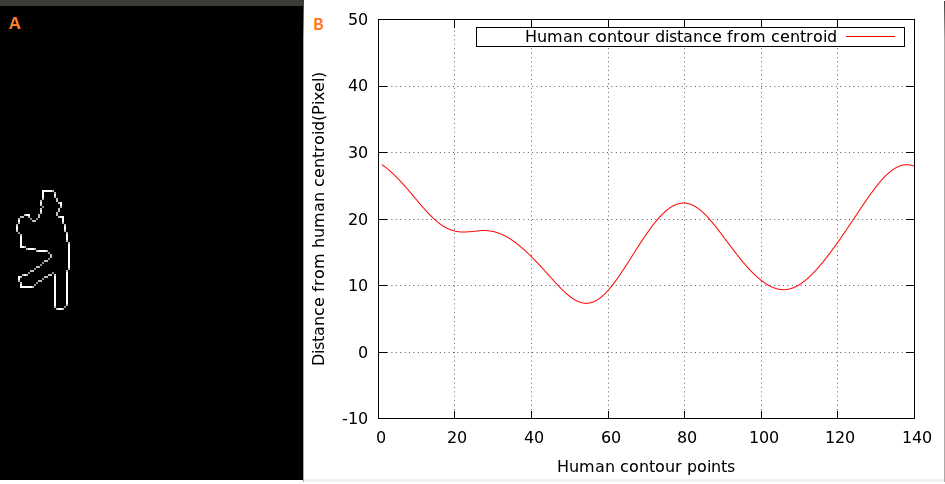
\includegraphics[height=200pt]{Figures/distance}
\caption{Distance plot of human contour points from its centroid}
\label{distance}
\end{figure}
\item Distance vector array is smoothed to remove noise peaks using
	cvSmooth. If these distances are plotted then it looks like
	Fig.~\ref{distance}. Now local maxima of distance vector is
	calculated by finding zero crossing of difference vectors. These
	local maxima provides a star form of skeleton centered at
	centroid of the object. A typical star skeleton has been shown
	in Fig.~\ref{skeletons}.C.
\end{itemize}
\end{itemize}
\subsection{Human detection methods}
\indent We have evaluated three methods of human detection technique mainly on the
basis of their computation efficiency.
\begin{itemize}
\item \textbf{Detection using covariance features:} We have used method
	implemented by Yao et al. ~\cite{19}. We have selected this
	method, because it has been widely referenced and also the
	source(C code) is available in public domain.
\item \textbf{Detection using Haar-like features:} We have evaluated
	work by Viola et al.~\cite{16, 17} which uses Haar-like
	features for human detection. Again, reason to evaluate this
	algorithm was same, that it has been widely discussed and
	referenced.
\item \textbf{Detection using skeleton motion features:} We have
	evaluated this method as it seems to be computationally very
	efficient.  We have done our own implementation in C to evaluate
	this method.  Human motion can be represented suitably by
	movement of legs. So, we use star skeletonization method which
	seems best suitable for human leg motion analysis. We have seen
	that star skeletonization gives us skeleton points in form of peak
	distance from centroid. However, some of these peak points are
	not of our interest. In our algorithm, we are using two most relevant
	peaks which are nearest to each bottom corner of bounding box of
	contour respectively. Only these two peaks along with centroid
	give us sufficient information to distinguish human from
	human, vehicle or animal etc.\\
\indent For human subjects, the two peaks correspond to the two legs of
human. For vehicles, the peaks correspond to the two extrema points of
lower portion of back and front.  When it is an animal, the peaks
correspond to front and back leg of animal.\\
\item Let P$_1$(X$_1$, Y$_1$), P$_2$(X$_2$, Y$_2$) and C(C$_x$, C$_y$)
are two peaks nearest to bottom right and bottom left corner and
centroid respectively. Let $\theta$ is the angle between the line
segments P$_1$C and P$_2$C, then $\theta$ can be calculated as
follows.\\
%
	\begin{equation}
	\theta = tan^{-1}[(Y_2 - C_y) / (X_2 - C_x)] \\ - tan^{-1}[(Y_1 - C_y) / (X_1 - C_x)]
	\end{equation}
%
\indent If variation of $\theta$ is plotted in respective frames for
human and vehicle then the resultant plot is as shown in
Fig.\ref{angle_plot}.  The observations from this plot is that for a
human subject, angle variation pattern is repeatable, and it is zero for
almost at regular intervals.  For vehicle, it is constant. The
experiment with images containing animal is yet to be done. For images
with animals in it, there are variations with repeatable patterns but
which never touch zero.  These criterion can be the basis to identify an
object, and to decide whether it is a human,vehicle or animal.

\begin{figure}[!t]
\centering
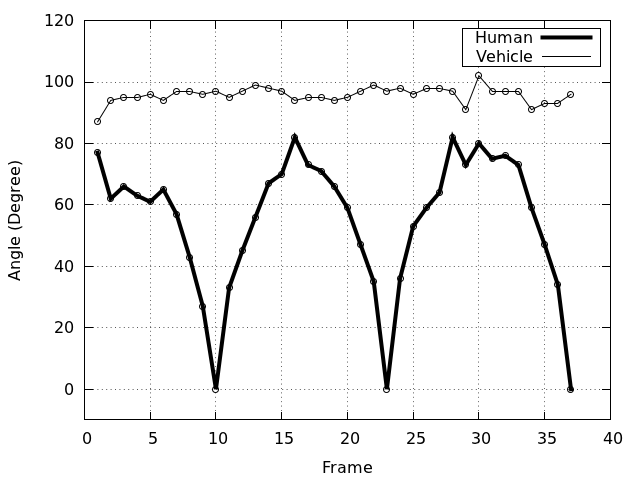
\includegraphics[height=300pt]{Figures/angle_plot}
\caption{Plot of variation of angle $\theta$ with frame number for human and
vehicle.}
\label{angle_plot}
\end{figure}
\item Every new object which comes into the field of view is tracked and
	value of (C$_x$, C$_y$), $\theta$ in each frame is stored. 
\begin{itemize} 
\item We track value of $\theta$ until it goes to zero three times.
\item Now we consider $\theta$ values between first and second zero as
vector T$_1$ and $\theta$ values between second and third zero as vector
T$_2$.
\item We find mean m$_1$ and m$_2$ of vector T$_1$ and T$_2$ respectively.
\item If n is the length of vector T$_1$ then, we calculate correlation
value (r) between these two vectors to find similarities as follows.
	\begin{equation}
	r = {{\Sigma ^n _{i = 1}(T_{1i} - m_1) . (T_{2i} - m_2)}
\over {\sqrt {\Sigma ^n _{i = 1} (T_{1i} - m_1)^2 . \Sigma ^n _{i = 1} (T_{2i}
- m_2)^2}}}
	\end{equation}
\item If correlation value is greater than a threshold value TH$_1$,
then we conclude that it is a human.
\end{itemize} 
\end{itemize} 
